% !TEX root = ./informe.tex

\section{Greedy}

\subsection{Explicación}

Vimos que construir la mejor solución de forma exacta es algo que, en la práctica, es completamente inutilizable por su complejidad temporal. Consideremos entonces la siguiente heurística: teniendo un conjunto solución $S$ que forma una clique, en cada paso podemos golosamente agregar a $S$ el mejor nodo que haga aumentar el tamaño de la frontera. \\

Intuitivamente es un algoritmo rápido, pues en cada iteración principal tomamos un nodo que forme clique con lo que ya tenemos, y ya no quitamos ese nodo. Además, parece razonable que el algoritmo encuentre soluciones buenas: en cada iteracion estamos maximizando la frontera con el mejor nodo posible. Luego de presentar el algoritmo veremos qué tan buena era nuestra intuición. \\

Mas detalladamente, el algoritmo funciona de la siguiente manera: \\

Primero consideramos que todos los nodos son candidatos, y vamos a ejecutar el algoritmo siempre que exista algún candidato en la lista. Además mantenemos un vector $S$ que representa la solución actual, inicialmente vacío. Consideramos que mi frontera máxima $FM$ inicia con valor $-1$. \\

Para cada iteracion del ciclo principal, queremos agregar el mejor candidato posible a la solución. Esto significa iterar por todos los candidatos y agregar a la solución aquel que maximice la frontera. \\

Recorremos la lista de candidatos y tomo alguno, $c$. Consideramos $c$ como parte de la solución. Si la solución $S$ no forma una clique, entonces quitamos $c$ de $S$ , consideramos que ya no es mas un candidato y volvemos al comienzo del algortimo. Si $S$ forma una clique, entonces calculamos su frontera $f$. \\

Comparamos la frontera $f$ con la frontera máxima $FM$. Si $f < FM$, entonces quitamos a $c$ de $S$, pues no hace que la solucion mejore. Si $f \geq FM$, entonces mantenemos a $c$, ahora $c$ es nuestro mejor candidato, pues la frontera máxima no empeoró. Actualizamos $FM$ con el valor de $f$. En ambos casos quitamos también a $c$ de la lista de candidatos, para no repetirlo dos veces. \\

Una vez encontrado el $c$ que maximice mi solución, lo agregamos definitivamente y seguimos iterando hasta que ya no se pueda considerar mas candidatos. \\

Finalizado el algoritmo, $S$ es una clique elegida de manera golosa, con la mayor frontera que se puedo encontrar. \\


\subsection{Pseudocódigo}

Referencias de variables globales para el pseudocódigo:
\begin{itemize}
    \item $n$: La cantidad de nodos
    \item $solucion$: Secuencia que contiene la clique solución
    \item $candidatos$: Secuencia con los nodos a considerar
    \item $fronteraMax$: El cardinal de la frontera de la clique solución
\end{itemize}

Las funciones ``EsClique()'' y ``Frontera()'' son las mismas que en el algortimo exacto. Dado que se usan en todos los algoritmos, son omitidas. Tienen complejidad $O(n^3)$ y $O(n^2)$ respectivamente.

\begin{algorithm}[H]
\begin{algorithmic}
\Function{Resolver}{}
    \State LeerInput()                              \Comment $O(n^2)$
    \State $solucion \gets \emptyset$               \Comment $O(1)$
    \State $candidatos \gets \{1, 2, 3, .. , n\} $  \Comment $O(n)$
    \State $fronteraMax \gets -1$                   \Comment $O(1)$
    \State ObtenerSolucion()                        \Comment $O(n^5)$
\EndFunction
\end{algorithmic}
\end{algorithm}



\begin{algorithm}[H]
\begin{algorithmic}
\Function{ObtenerSolucion}{}

    \While{$candidatos \neq \emptyset$}             \Comment $O(n^5)$

        \State $mejorCandidato \gets -1$            \Comment $O(1)$

        \For{$c \in candidatos$}                    \Comment $O(n^4)$
            \State $solucion.push(c)$               \Comment $O(1)$

            \If {$\neg$EsClique($solucion$)}                        \Comment $O(n^3)$
                \State $solucion.erase(c)$                          \Comment $O(n)$
                \State $candidatos.erase(c)$                        \Comment $O(n)$
            \Else
                \State $fronteraActual \gets$ Frontera($solucion$)  \Comment $O(n^2)$
                \If{$fronteraActual \geq fronteraMax$}              \Comment $O(1)$
                    \State $fronteraMax \gets fronteraActual$       \Comment $O(1)$
                    \State $mejorCandidato \gets c$                 \Comment $O(1)$
                \Else
                    \State $candidatos.erase(c)$                    \Comment $O(n)$
                \EndIf

                \State $solucion.erase(c)$                          \Comment $O(n)$
            \EndIf
        \EndFor

        \If{$mejorCandidato \neq -1$}                               \Comment $O(1)$
            \State $solucion.push(mejorCandidato)$                  \Comment $O(1)$
            \State $candidatos.erase(mejorCandidato)$               \Comment $O(n)$

        \EndIf
    \EndWhile

    \State return $solucion$

\EndFunction

\end{algorithmic}
\end{algorithm}

\subsection{Complejidad}

La complejidad principal del algoritmo se encuentra en ``ObtenerSolucion()'', que es $O(n^5)$. Esto es fácil de ver: como nunca se agregan candidatos y siempre se quita al menos uno, el ciclo exterior se ejecuta a lo sumo $O(n)$ veces. El $For$ recorre la lista de candidatos, que son tambien a lo sumo $O(n)$. Dentro del $For$ encontramos solo dos funciones grandes, ``EsClique'' de $O(n^3)$ y ``Frontera'' de $O(n^2)$. El resto son comparaciones, asignaciones y borrados, de $O(n)$. \\

Mas intuitivamente, EsClique ($O(n^3)$) se ejecuta $O(n)$ veces en el For, y a su vez se ejecuta $O(n)$ veces en el While. Por lo tanto, es $O(n^5)$. \\

Si bien $O(n^5)$ puede parecer un polinomio ``grande'', es exponencialmente mejor que el algortimo exacto que tenía $O(2^{n} * n^{3})$. El trade-off es que no siempre se producen soluciones óptimas, como veremos más adelante. \\

\subsection{Optimalidad}

Como podrá verse mas adelante, las soluciones para grafos aleatorios son bastante buenas, pero existe al menos un tipo específico de grafos donde la diferencia entre el exacto y el greedy puede ser \textbf{arbitrariamente grande}. \\

Veamos como podemos construir este tipo de grafos. Vamos a aprovecharnos de que el algoritmo greedy recorre los nodos en orden: 1, 2, 3, 4. \\

{\centering
    
\includegraphics[width=0.57\textwidth]{informe/imgs/greedy_base.png} \\
    \captionof{figure}{Grafo inicial}
}

$ $\newline

Agreguemos 6 vecinos al nodo 1 y agreguemos 4 vecinos a los nodos 2 y 3. El algoritmo goloso toma el primer nodo como solución inicial, es el que tiene mas vecinos. Luego intenta agregar nodos a la solucion de forma tal que formen clique y que tengan mayor frontera. Esto no puede suceder: lo mejor que puede obtener el algoritmo goloso es una clique con frontera de tamaño 7. Sin embargo, podemos ver que la solución óptima está formada por la clique con los nodos 2 y 3, con una frontera de tamaño 9.\\

{\centering
    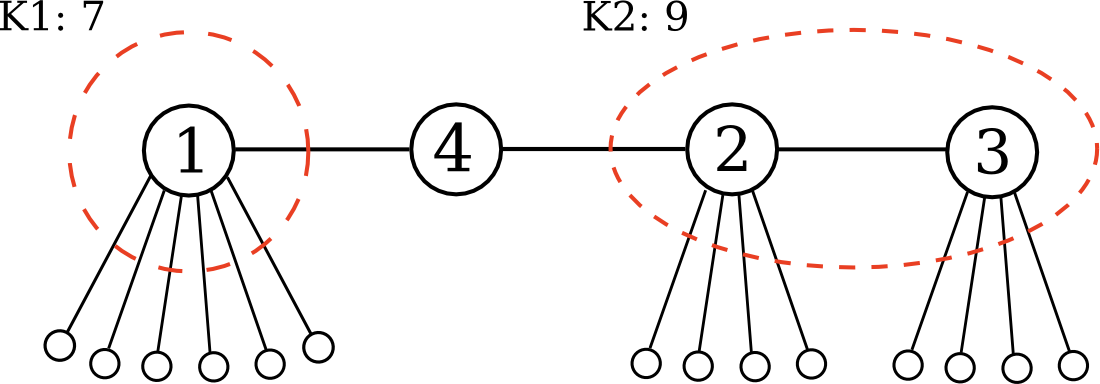
\includegraphics[width=0.57\textwidth]{informe/imgs/greedy_base_nodes_v1.png} \\
}
$ $\newline

Este es un procedimiento que podemos seguir repitiendo. Agregamos un vecino al nodo 1, y un vecino a los nodos 2 y 3. La frontera máxima golosa aumenta en 1, mientras que la frontera máxima aumenta en 2. De esta forma, podemos construir grafos donde la diferencia entre la solución óptima y la solución golosa sea arbitrariamente grande. \\

{\centering
    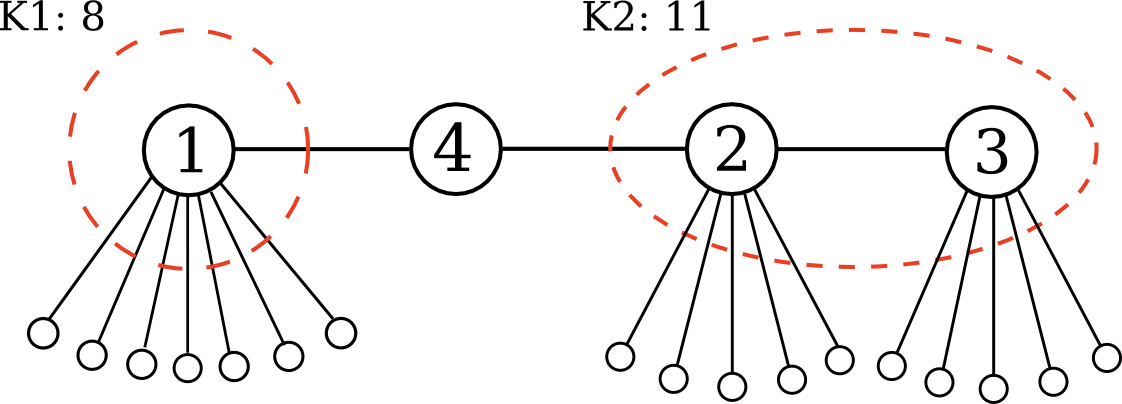
\includegraphics[width=0.57\textwidth]{informe/imgs/greedy_base_nodes_v2.png} \\
}

\subsection{Experimentación}


{\centering
    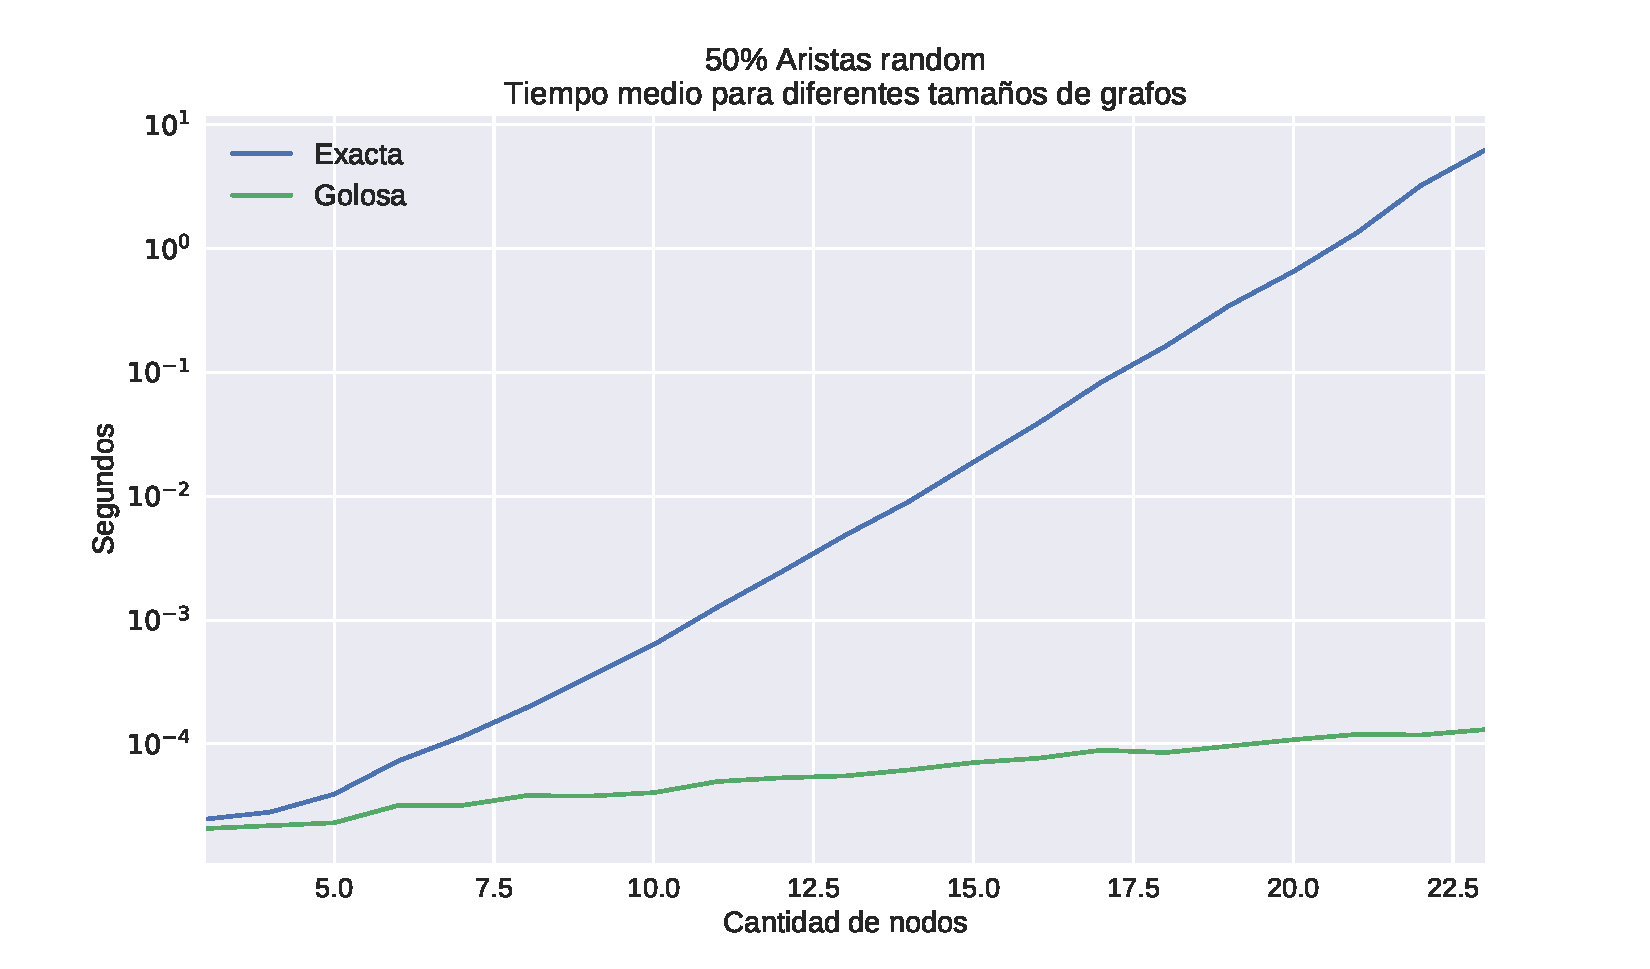
\includegraphics[width=1\textwidth]{informe/imgs/exp_random50_tiempo_greedy_exacta_logy.pdf} \\
       \captionof{figure}{Escala logarítmica}
}

{\centering
    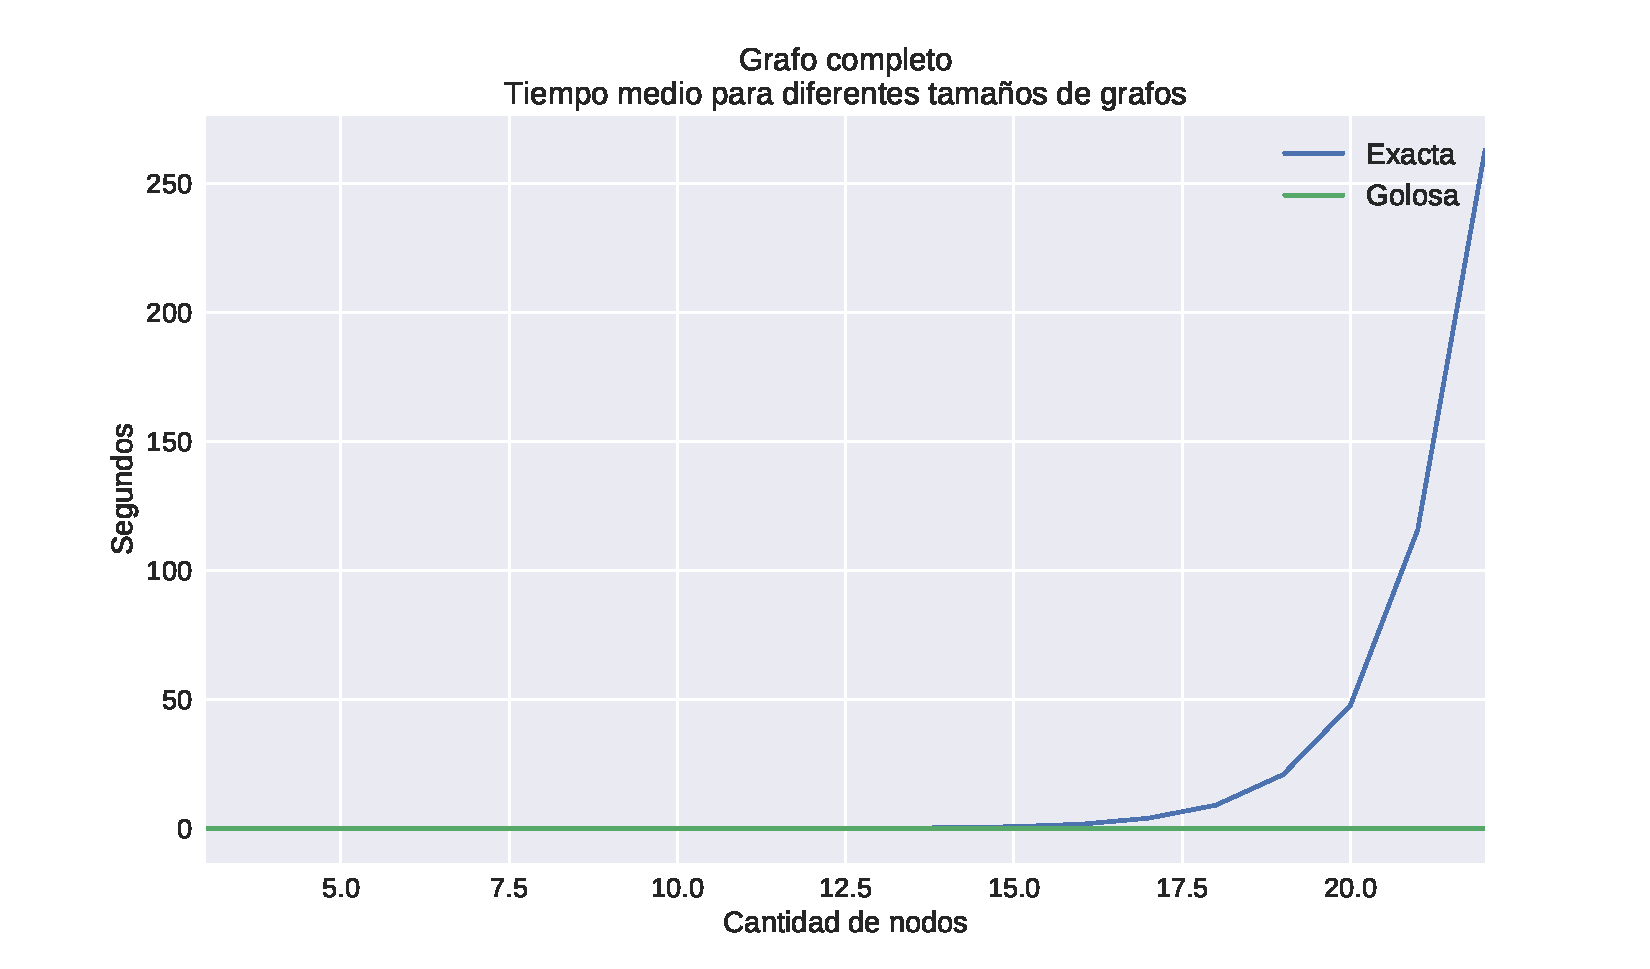
\includegraphics[width=1\textwidth]{informe/imgs/exp_completo_tiempo_greedy_exacta.pdf} \\
}

{\centering
    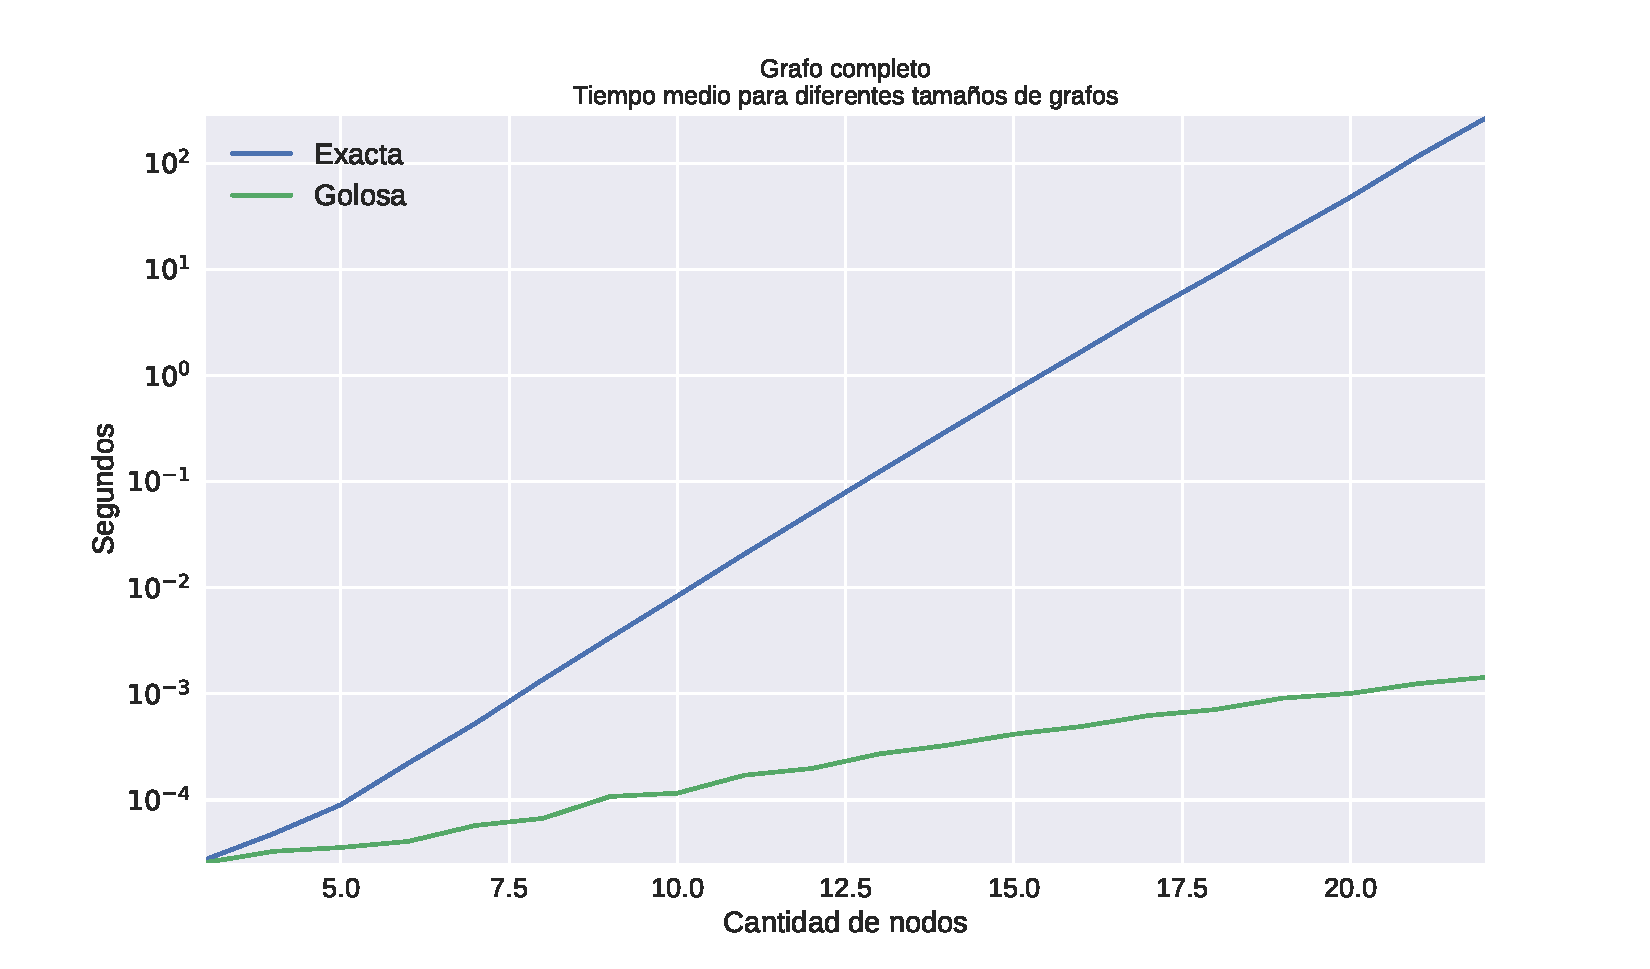
\includegraphics[width=1\textwidth]{informe/imgs/exp_completo_tiempo_greedy_exacta_logy.pdf} \\
    \captionof{figure}{Escala lagarítmica}
}

\todo[inline]{Dato de color, podemos ver el funcionamiento que el greedy toma cliques de menor tamaño, bla}

{\centering
    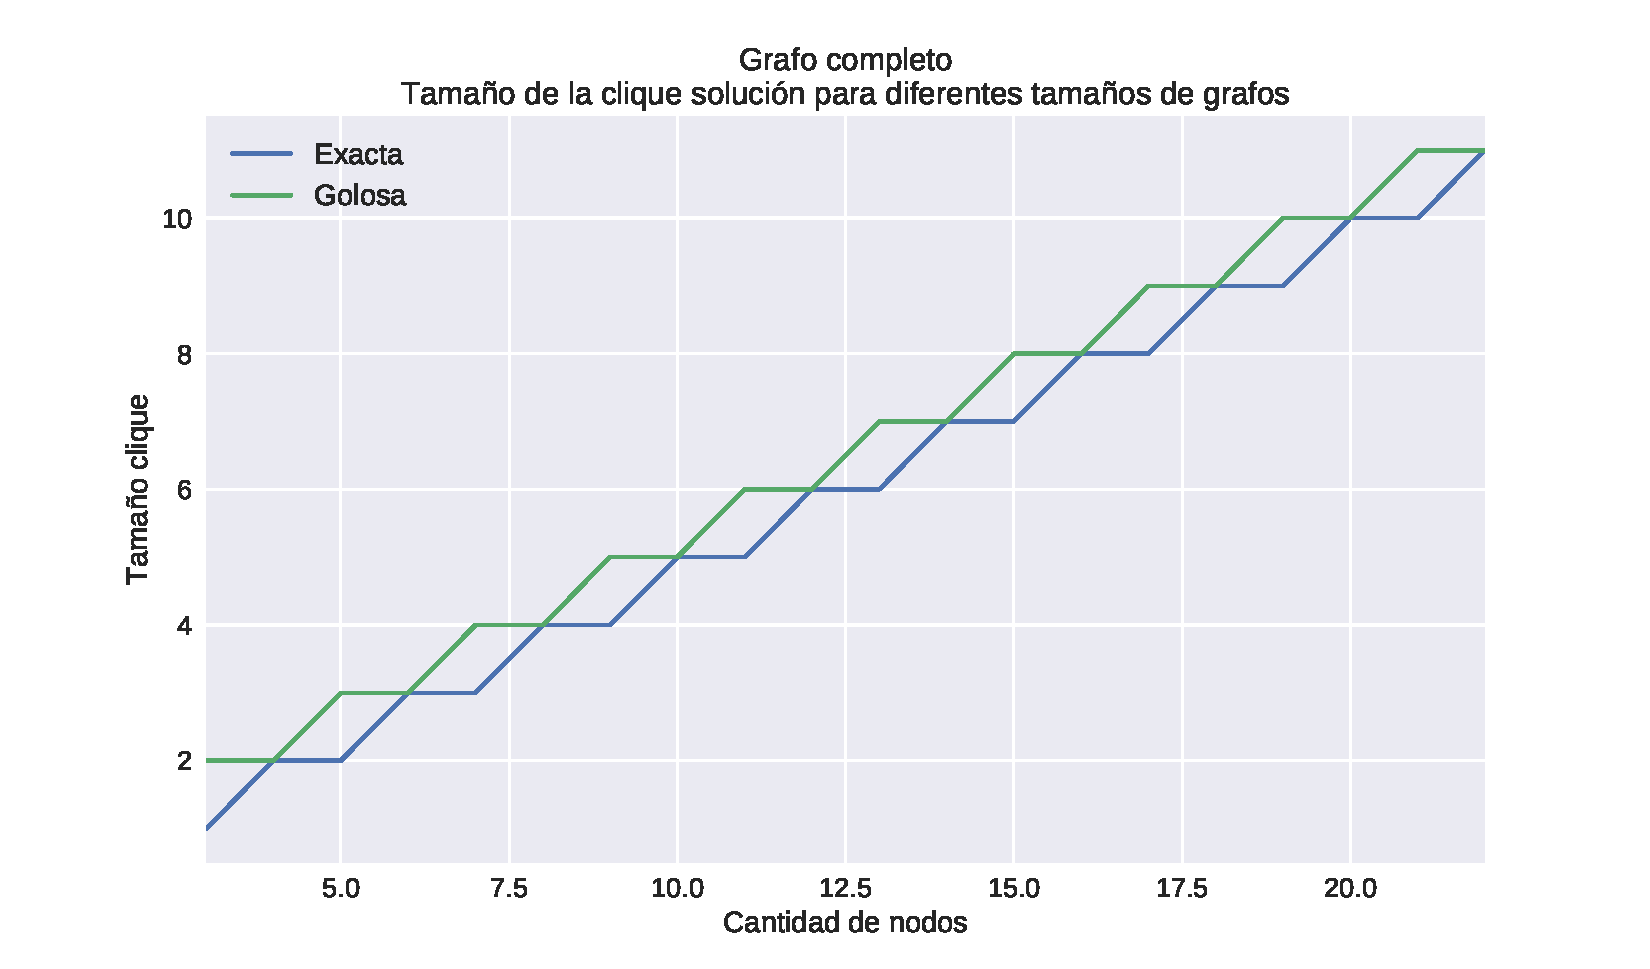
\includegraphics[width=1\textwidth]{informe/imgs/exp_completo_clique_greedy_exacta.pdf} \\
}

\todo[inline]{Volviendo a los casos malos, veamos que pasa con ellos. Como cambia la frontera.}

{\centering
    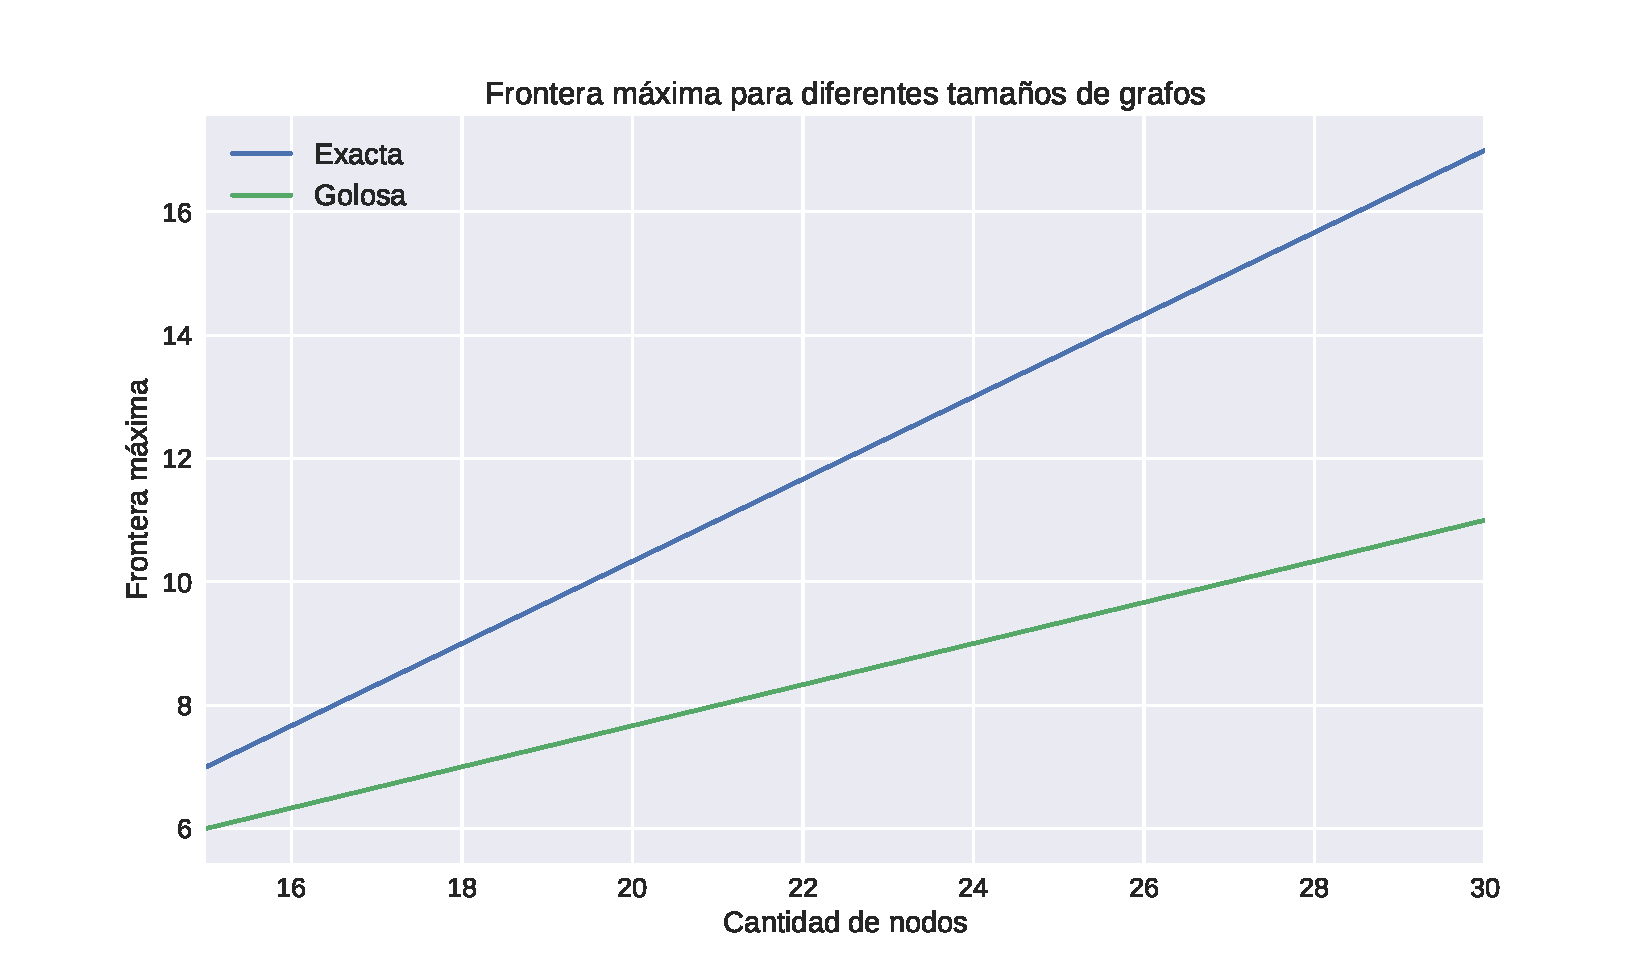
\includegraphics[width=1\textwidth]{informe/imgs/exp_malo_frontera_greedy_exacta.pdf} \\
    \captionof{figure}{Frontera para casos malos}
}

\todo[inline]{Conclusion: es super rapido, y en el caso promedio da muy buenas aproximaciones, pero existen casos muy muy malos. Veamos en las siguientes secciones como podemos solucionar este problema}